\begin{figure}
	\centering
	\pgfplotsset{every axis legend/.append style={
		at={(1.05,0.5)},
		anchor=west}}
	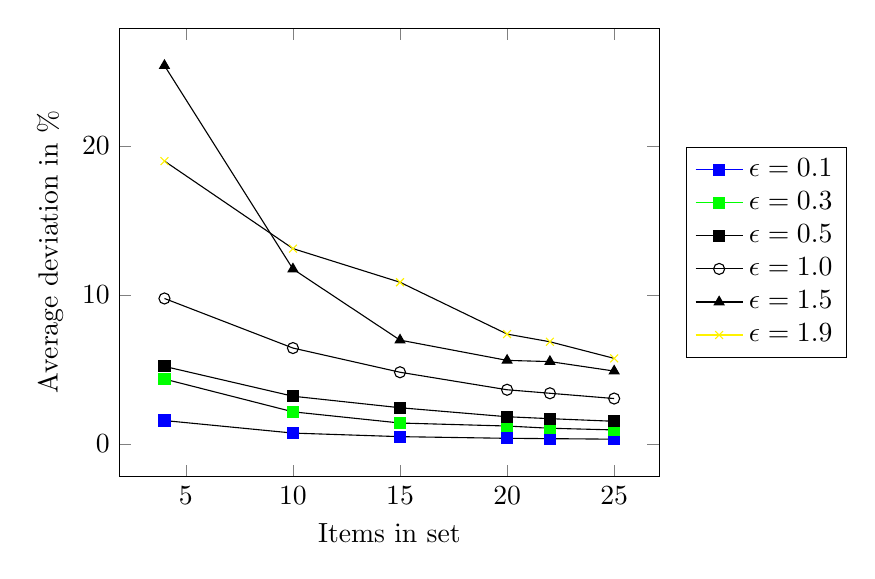
\begin{tikzpicture}
		\begin{axis}[
			xlabel=Items in set,
			ylabel=Average deviation in \%,
			scatter/classes={
				fptas1={mark=square*,blue},
				% fptas2={mark=square*,red},
				fptas3={mark=square*,green},
				% fptas4={mark=square*,yellow},
				fptas5={mark=square*,black},
				% fptas6={mark=o,blue},
				% fptas7={mark=o,red},
				% fptas8={mark=o,green},
				% fptas9={mark=o,yellow},
				fptas10={mark=o,black},
				% fptas11={mark=triangle*,blue},
				% fptas12={mark=triangle*,red},
				% fptas13={mark=triangle*,green},
				% fptas14={mark=triangle*,yellow},
				fptas15={mark=triangle*,black},
				% fptas16={mark=x,blue},
				% fptas17={mark=x,red},
				% fptas18={mark=x,green},
				fptas19={mark=x,yellow}
				}
            ]
            
\addplot[scatter,scatter src=explicit symbolic]table[meta=label] {
x y label
4 1.578520 fptas1
10 .736840 fptas1
15 .496943 fptas1
20 .385481 fptas1
22 .363280 fptas1
25 .327072 fptas1
};
\addplot[scatter,scatter src=explicit symbolic]table[meta=label] {
x y label
4 4.362344 fptas3
10 2.163470 fptas3
15 1.411930 fptas3
20 1.210040 fptas3
22 1.060910 fptas3
25 .949049 fptas3
};
\addplot[scatter,scatter src=explicit symbolic]table[meta=label] {
x y label
4 5.212682 fptas5
10 3.210590 fptas5
15 2.438080 fptas5
20 1.833507 fptas5
22 1.704880 fptas5
25 1.528040 fptas5
};
\addplot[scatter,scatter src=explicit symbolic]table[meta=label] {
x y label
4 9.771065 fptas10
10 6.443160 fptas10
15 4.819690 fptas10
20 3.644278 fptas10
22 3.408830 fptas10
25 3.055040 fptas10
};
\addplot[scatter,scatter src=explicit symbolic]table[meta=label] {
x y label
4 25.401756 fptas15
10 11.745500 fptas15
15 6.976230 fptas15
20 5.615681 fptas15
22 5.535220 fptas15
25 4.898940 fptas15
};
\addplot[scatter,scatter src=explicit symbolic]table[meta=label] {
x y label
4 18.992468 fptas19
10 13.119000 fptas19
15 10.859700 fptas19
20 7.381382 fptas19
22 6.864850 fptas19
25 5.750920 fptas19
};

			\addlegendentry{$\epsilon = 0.1$}
			\addlegendentry{$\epsilon = 0.3$}
			\addlegendentry{$\epsilon = 0.5$}
			\addlegendentry{$\epsilon = 1.0$}
			\addlegendentry{$\epsilon = 1.5$}
			\addlegendentry{$\epsilon = 1.9$}
		\end{axis}
	\end{tikzpicture}
\caption{Average deviation for maximal deviation}
\label{plot:devFptas}
\end{figure}
